\documentclass{beamer}
\usepackage[utf8]{inputenc}
\usepackage[english]{babel}

% -- Including some standard packages --
\usepackage{graphicx}
\usepackage{soul}
\usepackage{hyperref}
\usepackage{colortbl}
\usepackage{dsfont}
\usepackage{soul}

% -- Choosing theme --

\usetheme{Boadilla}
\usecolortheme{whale}
\setbeamercolor{alerted text}{fg=purple} % Making alerted text non-red

% Tikz
\usepackage{tikz}
\usetikzlibrary{matrix,positioning,fit,backgrounds,intersections}

% -- Cross signs --
\usepackage{pifont} % http://ctan.org/pkg/pifont
\newcommand{\cmark}{\ding{51}}%
\newcommand{\xmark}{\ding{55}}%
\newcommand{\xopt}{\ding{48}}%

% -- Custom commands --
\DeclareMathOperator*{\argmax}{arg\,max}
\DeclareMathOperator*{\argmin}{arg\,min}

\title[Mathematics I]{\textbf{Mathematics for Cryptography: Number Theory, Groups, Polynomials}}
\author{Distributed Lab}
\date{July 18, 2024}
\titlegraphic{
    
\includegraphics[width=\textwidth]{images/banner_wide.png}
}

\expandafter\def\expandafter\insertshorttitle\expandafter{%
  \insertshorttitle\hfill%
  \insertframenumber\,/\,\inserttotalframenumber}

\AtBeginSection[]{
  \begin{frame}
  \vfill
  \centering
  \begin{beamercolorbox}[sep=8pt,center,shadow=true,rounded=true]{title}
    \usebeamerfont{title}\insertsectionhead\par%
  \end{beamercolorbox}
  \vfill
  \end{frame}
}

\begin{document}
    \frame {
      \titlepage
    }
  
    \begin{frame}{Plan}
      \tableofcontents
    \end{frame}

    \section{Some words about the course}
    \begin{frame}{About ZKDL} 

      \begin{columns}
        % Description
        \begin{column}{0.7\textwidth}
          \begin{itemize}
            \item ZKDL is an intensive course on low-level zero-knowledge cryptography.
            \item We will learn zero-knowledge proving systems \textbf{from total scratch}.
            \item This means that the material is \textbf{hard}. We want commitment and attention from your side.
            \item We, in turn, provide you structured explanation of the material, practical examples and exercises.
          \end{itemize}
        \end{column}
        % Column 2    
        \begin{column}{0.3\textwidth}
            \begin{figure}
            \centering
                
\includegraphics[width=1\textwidth]{images/logo.png}
            \end{figure}
        \end{column}
        \end{columns}

      \begin{alertblock}{Note}
        This course is beneficial for everyone: even lecturers do not know all the material and content is subject to change. Please, feel free to ask questions and provide feedback, and we will adjust the material accordingly.
      \end{alertblock}

    \end{frame}

    \begin{frame}{Why ZKDL?}

      \begin{columns}
        % Description
        \begin{column}{0.65\textwidth}
          \begin{itemize}
            \item Better Mathematics understanding.
            \item Skill of reading academic papers and writing your own ones.
            \item Public speech skills for lecturers on complex topics.
            \item Our knowledge structurization condensed in one course.
            \item Importance of ZK is quite obvious.
            \item And, of course, cryptography is fun!
          \end{itemize}
        \end{column}
        % Column 2    
        \begin{column}{0.35\textwidth}
            \begin{figure}
            \centering
                
\includegraphics[width=\textwidth]{images/lecture_1/thonk.png}
            \end{figure}
        \end{column}
        \end{columns}
        
        \begin{alertblock}{Note}
          We are R\&D experts in Cryptography, so we need to boost our skills in academic writing, lecturing, and understanding very advanced topics.
        \end{alertblock}
    \end{frame}

    \begin{frame}{Format}
      \begin{enumerate}
        \item We will gather every Thursday at 7PM.
        \item Lecturer will be different based on the topic.
        \item We will send you the lecture notes beforehand. Highly recommended to read it before the lecture.
        \item We also attach exercises, which are highly recommended. You might ask questions about them during the lecture.
        \item \textit{Optionally}, we will conduct workshops on a separate day. We will discuss this later.
      \end{enumerate}
    \end{frame}

    \begin{frame}{Contents}

      \begin{columns}
        % Description
        \begin{column}{0.65\textwidth}
          \begin{enumerate}
            \item Mathematics Preliminaries: group and number theory, finite fields, polynomials, elliptic curves etc.
            \item Building SNARKs from scratch.
            \item Analysis of modern zero-knowledge proving systems: Groth16, Plonk, BulletProofs, STARK etc.
            \item Specialization topics: low-level optimizations, advanced protocols such as folding schemes, Nova etc.
          \end{enumerate}
        \end{column}
        % Column 2    
        \begin{column}{0.35\textwidth}
            \begin{figure}
            \centering
                
\includegraphics[width=\textwidth]{images/lecture_1/blender.png}
            \end{figure}
        \end{column}
        \end{columns}
    \end{frame}

    \section{Notation}

    \subsection{Sets}

    \begin{frame}{Sets}
      \begin{definition}
        \textbf{Set} is a collection of \textit{distinct} objects, considered as an object in its own right.
      \end{definition}

      \begin{example}
        \begin{itemize}
          \item $\mathbb{N}$ is a set of natural numbers.
          \item $\mathbb{Z}$ is a set of integers.
          \item $\mathbb{R}$ is a set of real numbers.
          \item $\mathbb{R}_{>0}$ is a set of positive real numbers.
          \item $\{1, 2, 5, 10\}$ is a set of four elements.
          \item $\{1, 2, 2, 3\} = \{1,2,3\}$ -- we do not count duplicates.
          \item $\{1,2,3\} = \{2,1,3\}$ -- order does not matter.
        \end{itemize}
      \end{example}
    \end{frame}

    \begin{frame}{Operations on sets}
    % --- Writing diagrams ---
    \def\firstcircle{(0,0) circle (1.5cm)}
    \def\secondcircle{(0:2cm) circle (1.5cm)}

    \colorlet{circle edge}{blue!50}
    \colorlet{circle area}{blue!20}

    \tikzset{filled/.style={fill=circle area, draw=circle edge, ultra thick},
        outline/.style={draw=circle edge, ultra thick}}    

      \begin{figure}
        \begin{center}
        \begin{tabular}{cc}
        % Set A and B
        \begin{tikzpicture}
            \begin{scope}
                \clip \firstcircle;
                \fill[filled] \secondcircle;
            \end{scope}
            \draw[outline] \firstcircle node {$A$};
            \draw[outline] \secondcircle node {$B$};
            \node[anchor=south] at (current bounding box.north) {$A \cap B$};
        \end{tikzpicture} &   
        %Set A or B but not (A and B) also known a A xor B
        \begin{tikzpicture}
            \draw[filled, even odd rule] \firstcircle node {$A$}
                                        \secondcircle node{$B$};
            \node[anchor=south] at (current bounding box.north) {$\overline{A \cap B}$};
        \end{tikzpicture}
        \\
        % Set A or B
        \begin{tikzpicture}
            \draw[filled] \firstcircle node {$A$}
                        \secondcircle node {$B$};
            \node[anchor=south] at (current bounding box.north) {$A \cup B$};
        \end{tikzpicture} &  
        % Set A but not B
        \begin{tikzpicture}
            \begin{scope}
                \clip \firstcircle;
                \draw[filled, even odd rule] \firstcircle node {$A$}
                                            \secondcircle;
            \end{scope}
            \draw[outline] \firstcircle
                        \secondcircle node {$B$};
            \node[anchor=south] at (current bounding box.north) {$A \setminus B$};
        \end{tikzpicture}
    \end{tabular}
    \end{center}
    \label{fig:venn_diagrams}
    \end{figure}
    \end{frame}
    
    \begin{frame}{Defining sets}
      \begin{example}
        \begin{itemize}
          \item $\{x \in \mathbb{R}: x^2 = 1\}$ -- a set of real numbers that satisfy the equation $x^2 = 1$.
          \item $\{x \in \mathbb{Z}: x \text{ is even}\}$ -- a set of even integers.
          \item $\{x^2: x \in \mathbb{R}, x^3 = 1\}$ -- a set of squares of real numbers that satisfy the equation $x^3 = 1$.
          \item $\{x \in \mathbb{N}: x \text{ is prime}\} \setminus \{2\}$ -- a set of odd prime numbers.
        \end{itemize}
      \end{example}

      \begin{alertblock}{Question \#1}
        How to simplify the set $\{x \in \mathbb{N}: x^2 = 2\}$?
      \end{alertblock}
  
      \begin{alertblock}{Question \#2(*)}
        How to simplify the set $\{\sin \pi k: k \in \mathbb{Z}\}$?
      \end{alertblock}
    \end{frame}

    \subsection{Logic}
    \begin{frame}{Basic Logic}
        \begin{itemize}
          \item $\forall$ means ``for all''.
          \item $\exists$ means ``there exists'', $\exists!$ means ``there exists the only''.
          \item $\land$ means ``and''.
          \item $\lor$ means ``or''.
        \end{itemize}

        \begin{alertblock}{Question \#1}
            Is it true that $(\forall x \in \mathbb{N}): \{x > 0\}$?
        \end{alertblock}

        \begin{alertblock}{Question \#2}
            Is it true that $(\exists x \in \mathbb{N}): \{x \geq 0 \land x < 1\}$?
        \end{alertblock}

        \begin{alertblock}{Question \#3}
            Is it true that $(\forall x \in \mathbb{Z})\, (\exists y \in \mathbb{N}): \{y > x\}$?
        \end{alertblock}
    \end{frame}

    \subsection{Randomness and Sequences}

    \begin{frame}{Randomness and Sequences}
        \begin{block}{Notation}
          To denote probability of event $E$, we use notation $\text{Pr}[E]$. For example,
          \begin{equation*}
              \text{Pr}[\text{It will be cold tomorrow}] = 0
          \end{equation*}
        \end{block}

        \begin{block}{Notation}
            To denote that we take an element from a set $S$ uniformly at random, we use notation $x \xleftarrow{R} S$.

            For example, when throwing a coin, we can write $x \xleftarrow{R} \{\text{heads}, \text{tails}\}$.
        \end{block}

        \begin{block}{Notation}
          To denote an infinite sequence $x_1,x_2,\cdots$, we use $\{x_i\}_{i \in \mathbb{N}}$. To denote
          a finite sequence $x_1,x_2,\cdots,x_n$, we use $\{x_i\}_{i=1}^n$. To enumerate 
          through a list of indeces $\mathcal{I} \subset \mathbb{N}$, we use notation
          $\{x_i\}_{i \in \mathcal{I}}$.
        \end{block}
    \end{frame}

    \section{Basic Group Theory}

    \subsection{Reasoning behind Groups}
    \begin{frame}{Why Groups?!}
        Well, first of all, we want to work with integers\ldots

        Imagine that Alice pays to Bob with a card number $N$, but instead of paying to a number $N$, the system pays 
        to another card number $N+k, k \ll N$, which is only by 0.001\% different. Bob would not be 99.999\% happy\ldots

        \begin{figure}
          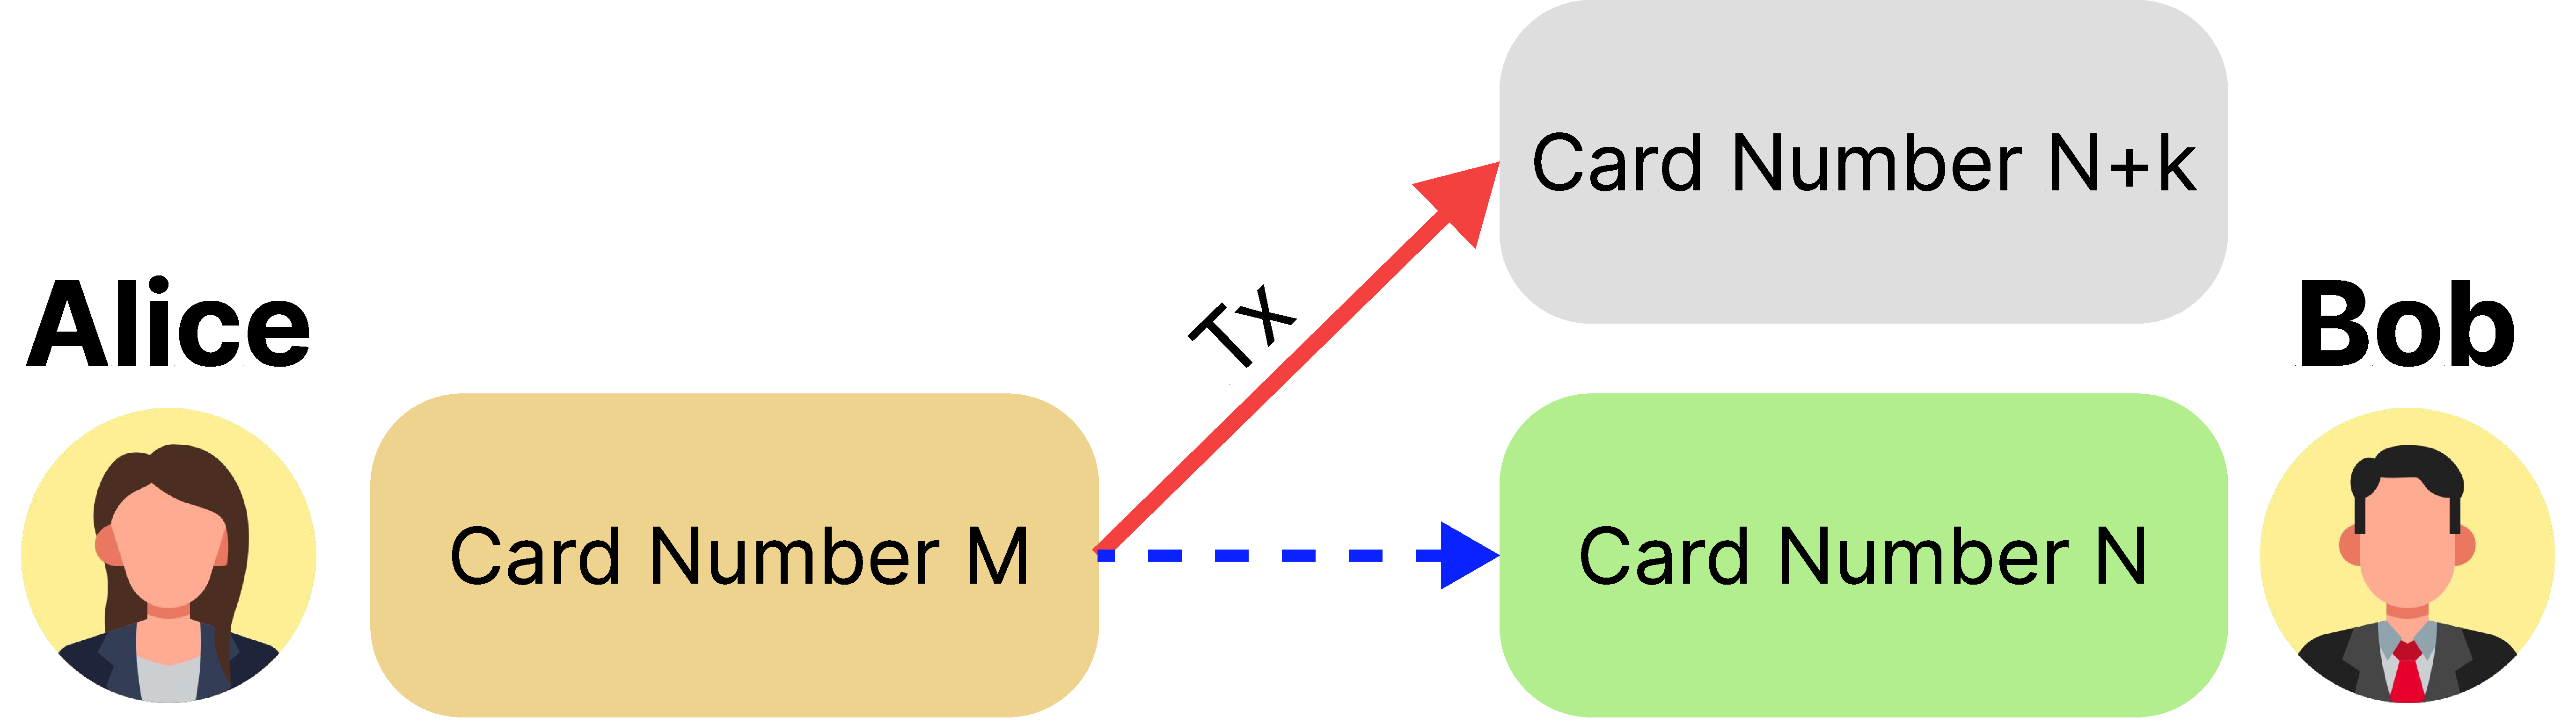
\includegraphics[width=1.0\textwidth]{images/lecture_1/why_integers.pdf}
          \label{fig:why_integers}
        \end{figure}
    \end{frame}

    \begin{frame}{Why Groups?!}
        But integers on their own are not enough. We need to define a structure that allows us to perform operations on them.

        This is very similar to interfaces: we abstract from the implementation, just merely stating we have ``some'' addition/multiplication.

        \begin{example}
            Consider set $\mathbb{G} := \{\text{Dmytro}, \text{Dan}, \text{Friendship}\}$. We can safely define an operation $\oplus$ as:
            \begin{gather*}
                \text{Dmytro} \oplus \text{Dan} = \text{Friendship} \\ 
                \text{Dan} \oplus \text{Friendship} = \text{Dmytro} \\
                \text{Friendship} \oplus \text{Dmytro} = \text{Dan}
            \end{gather*}
        \end{example}

        \begin{block}{Rhetorical question}
            What makes $(\mathbb{G}, \oplus)$ a group?
        \end{block}
    \end{frame}
    \subsection{Group Definition and Examples}
    \begin{frame}{Group Definition}
      \begin{definition}
        \textbf{Group} $(\mathbb{G}, \oplus)$, is a set with a binary operation $\oplus$ with following rules:
        \begin{enumerate}
            \item \textbf{Closure:} Binary operations always outputs an element from $\mathbb{G}$, that is $\forall a,b \in \mathbb{G}: a \oplus b \in \mathbb{G}$.
            \item \textbf{Associativity:} $\forall a,b,c \in \mathbb{G}: (a \oplus b)\oplus c = a \oplus (b \oplus c)$.
            \item \textbf{Identity element:} There exists a so-called identity element $e \in \mathbb{G}$ such that $\forall a \in \mathbb{G}: e \oplus a = a \oplus e = a$.
            \item \textbf{Inverse element:} $\forall a \in \mathbb{G} \; \exists b \in \mathbb{G}: a\oplus b = b \oplus a = e$. We commonly denote the inverse element as $(\ominus a)$.
        \end{enumerate}
    \end{definition}

    \begin{definition}
        A group is called \textbf{abelian} if it satisfies the additional rule called \textbf{commutativity}: $\forall a,b \in \mathbb{G}: a \oplus b = b \oplus a$.
    \end{definition}
    \end{frame}

    \begin{frame}{Explanation for Developers: Trait}
      \begin{center}
        \begin{figure}
          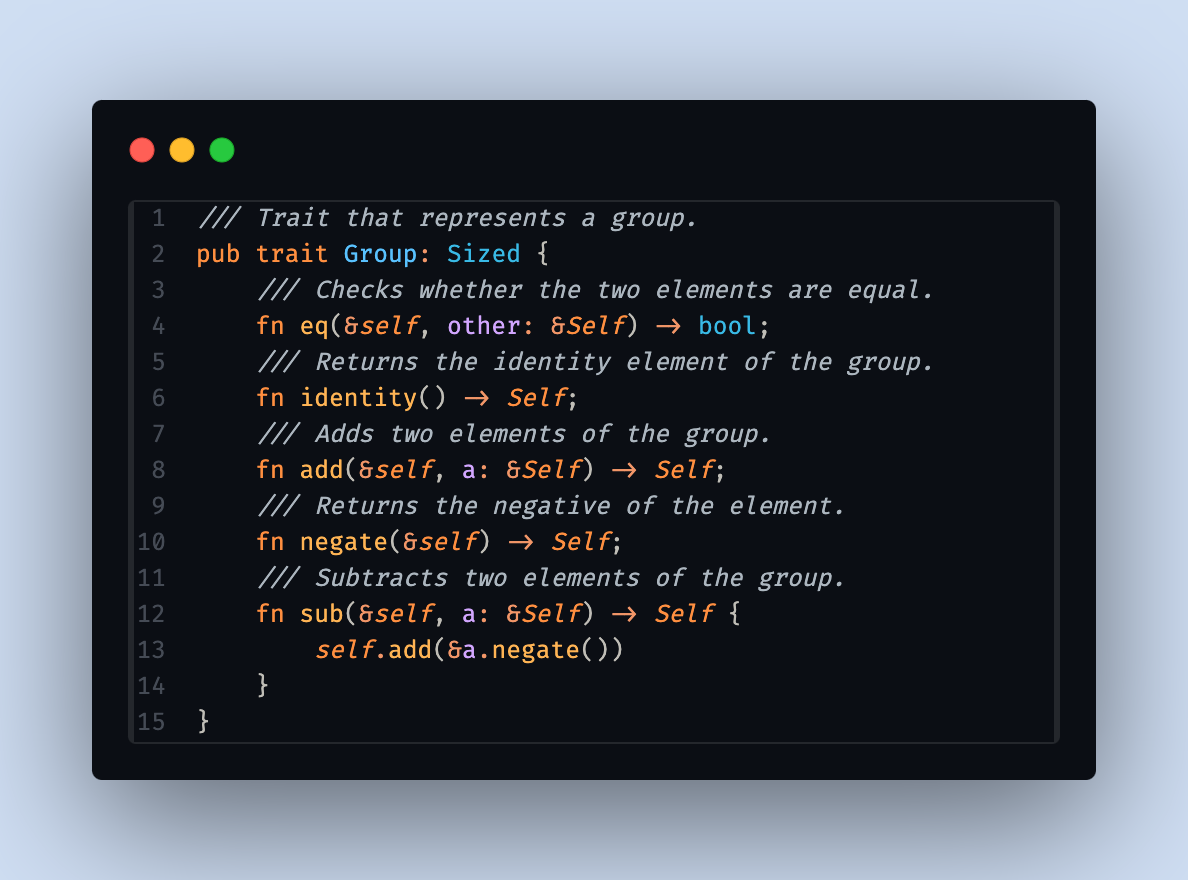
\includegraphics[width=0.8\textwidth]{images/lecture_1/group_in_rust.png}
          \label{fig:group_in_rust}
        \end{figure}

        More on that: \url{https://github.com/ZKDL-Camp/lecture-1-math}.
      \end{center}
    \end{frame}

    \begin{frame}{Group Examples}
      \begin{example}
        A group of integers with the regular addition $(\mathbb{Z},+)$ (also called the \textit{additive} group of integers) is a group.
      \end{example}
      
      \begin{example}
          The multiplicative group of positive real numbers $(\mathbb{R}_{> 0}, \times)$ is a group for similar reasons. 
      \end{example}
      
      \begin{alertblock}{Question \#1}
          Is $(\mathbb{R}, \times)$ a group? If no, what is missing?
      \end{alertblock}

      \begin{alertblock}{Question \#2}
        Is $(\mathbb{Z}, \times)$ a group? If no, what is missing?
      \end{alertblock}
    \end{frame}

    \begin{frame}{Small Note on Notation}
      \begin{block}{Additive group}
          We say that a group is \textit{additive} if the operation is denoted as $+$, and the identity element is denoted as $0$.
      \end{block}

      \begin{block}{Multiplicative group}
          We say that a group is \textit{multiplicative} if the operation is denoted as $\times$, and the identity element is denoted as $1$.
      \end{block}
      \begin{block}{Rule of thumb}
        We use additive notation when we imply that the group $\mathbb{G}$ is the set of points on the elliptic curve, while multiplicative is typically used in the rest of the cases.
      \end{block}
  \end{frame}

    \begin{frame}{Abelian Groups Examples and Non-Examples}
      \begin{alertblock}{Question \#3}
        Is $(\mathbb{R}, -)$ a group? If no, what is missing?
      \end{alertblock}
      \begin{alertblock}{Question \#4}
          Set $V$ is a set of tuples $(v_1,v_2,v_3)$ where each $v_i \in \mathbb{R} \setminus \{0\}$. Define the operation $\odot$ as
          \begin{equation*}
              (v_1,v_2,v_3) \odot (u_1,u_2,u_3) = (v_1u_1, v_2u_2, v_3u_3)
          \end{equation*}

          Is $(V, \odot)$ a group? If no, what is missing?
      \end{alertblock}
      \begin{block}{Conclusion}
        Group is just a fancy name for a set with a binary operation that behaves nicely.
      \end{block}
    \end{frame}

    \subsection{Subgroup}
    \begin{frame}{Subgroup}

      \begin{alertblock}{Question}
          Suppose $(\mathbb{G}, \oplus)$ is a group. Is any subset $\mathbb{H} \subset \mathbb{G}$ a group?
      \end{alertblock}

      \begin{definition}
          A \textbf{subgroup} is a subset $\mathbb{H} \subset \mathbb{G}$ that is a group with the same operation $\oplus$. We denote it as $\mathbb{H} \leq \mathbb{G}$.
      \end{definition}

      \begin{example}
          Consider $(\mathbb{Z}, +)$. Then, although $\mathbb{N} \subset \mathbb{Z}$, it is not a subgroup, as it does not have inverses.
      \end{example}

      \begin{example}
          Consider $(\mathbb{Z}, +)$. Then, $3\mathbb{Z} = \{3k: k \in \mathbb{Z}\} \subset \mathbb{Z}$ is a subgroup.
      \end{example}
  \end{frame}

  \begin{frame}{Questions}
    \begin{alertblock}{Question \#1}
      Does any group have at least one subgroup?
    \end{alertblock}

    \textbf{Answer.} Yes, take $\mathbb{H} = \{e\} \leq \mathbb{G}$.

    \begin{alertblock}{Question \#2*}
      Let $\mathsf{GL}(\mathbb{R},2)$ be a mutliplicative group of invertable matrices, while $\mathsf{SL}(\mathbb{R},2)$ be a multiplicative group of matrices with determinant 1. Is $\mathsf{SL}(\mathbb{R},2) \leq \mathsf{GL}(\mathbb{R},2)$?
    \end{alertblock}

    \textbf{Answer.} Yes. For $A = \begin{bmatrix}
      a & b \\
      c & d
    \end{bmatrix} \in \mathsf{SL}(\mathbb{R},2)$ the inverse is $A^{-1} = \begin{bmatrix}
      d & -b \\ -c & a
    \end{bmatrix}$. Also, $\det (AB) = \det A \cdot \det B$, so the product of two matrices with determinant 1 has determinant 1, so the operation in closed.
  \end{frame}

  \subsection{Homomorphism and Isomorphism}

  \begin{frame}{Homomorphism}
    \begin{definition}
      A \textbf{homomorphism} is a function $\phi: \mathbb{G} \rightarrow \mathbb{H}$ between two groups $(\mathbb{G}, \oplus)$ and $(\mathbb{H}, \odot)$ that preserves the group structure, i.e., 
      \begin{equation*}
        \forall a,b \in \mathbb{G}: \phi(a \oplus b) = \phi(a) \odot \phi(b)
      \end{equation*}
    \end{definition}

    \begin{example}
      Consider $(\mathbb{Z}, +)$ and $(\mathbb{R}_{>0}, \times)$. Then, the function $\phi: \mathbb{Z} \rightarrow \mathbb{R}_{>0}$ defined as $\phi(k) = 2^k$ is a homomorphism.
    \end{example}

    \textbf{Proof}. Take any $n,m \in \mathbb{Z}$ and consider $\phi(n+m)$:
    \begin{equation*}
      \phi(n+m) = 2^{n+m} = 2^n \times 2^m = \phi(n) \times \phi(m)
    \end{equation*}
  \end{frame}

  \begin{frame}{Mapping types}
    \begin{figure}
      \includegraphics[width=0.7\textwidth]{images/lecture_1/mapping.pdf}
      \label{fig:mappings}
    \end{figure}
  \end{frame}

  \begin{frame}{Homomorphism}
    \begin{definition}
      \textbf{Isomorphism} is a bijective homomorphism.
    \end{definition}

    \begin{definition}
      Two groups $\mathbb{G}$ and $\mathbb{H}$ are \textbf{isomorphic} if there exists an isomorphism between them. We denote it as $\mathbb{G} \cong \mathbb{H}$.
    \end{definition}

    \begin{example}
     $\phi: k \mapsto 2^k$ from the previous example is a homomorphism between $(\mathbb{Z},+)$ and $(\mathbb{R}_{>0},\times)$, but not an isomorphism. Indeed, there is no $x \in \mathbb{Z}$ such that $2^x = 3 \in \mathbb{R}_{>0}$.
    \end{example}

    \begin{alertblock}{Question}
      What can we do to make $\phi$ an isomorphism?
     \end{alertblock}
  \end{frame}

  \begin{frame}{Field}
    \begin{block}{Informal Definition}
        \textbf{Field} $\mathbb{F}$ is a set equipped with appropriate \textbf{addition} and \textbf{multiplication} operations with the corresponding well-defined inverses, where you can perform the basic arithmetic.
    \end{block}
    
      \begin{definition}
        A \textbf{field} is a set $\mathbb{F}$ with two operations $\oplus$ and $\odot$ such that:
        \begin{enumerate}
            \item $(\mathbb{F}, \oplus)$ is an abelian group with identity $e_{\oplus}$.
            \item $(\mathbb{F} \setminus \{e_{\oplus}\}, \odot)$ is an abelian group.
            \item The \textbf{distributive law} holds: $\forall a,b,c \in \mathbb{F}: a \odot (b \oplus c) = (a \odot b) \oplus (a \odot c)$.
        \end{enumerate}
      \end{definition}
    \end{frame}

    \begin{frame}{Field Examples}
      \begin{example}
        The set of real numbers $(\mathbb{R}, +, \times)$ is obviously a field. So is $(\mathbb{Q}, +, \times)$.
    \end{example}

    \begin{definition}
      \textbf{Finite Field} is the set $\{0,\dots,p-1\}$ equipped with operations modulo $p$ is a field if $p$ is a prime number.
    \end{definition}

    \begin{example}
      The set $\mathbb{F}_5 = \{0,1,2,3,4\}$ with operations modulo $5$ is a field. Operation examples:
      \begin{itemize}
        \item $3 + 4 = 2$.
        \item $3 \times 2 = 1$.
        \item $4^{-1} = 4$ since $4 \times 4 = 1$.
      \end{itemize}
    \end{example}
    \end{frame}

    \section{Polynomials}

    \subsection{Definition}

    \begin{frame}{Definition}
      \begin{definition}
        A \textbf{polynomial} $f(x)$ is a function of the form
        \begin{equation*}
            p(x) = c_0 + c_1 x + c_2 x^2 + \cdots + c_n x^n = \sum_{k=0}^{n} c_k x^k,
        \end{equation*}
        where $c_0, c_1, \dots, c_n$ are coefficients of the polynomial.
    \end{definition}
    
    \begin{definition}
        A set of polynomials depending on $x$ with coefficients in a field $\mathbb{F}$ is denoted as $\mathbb{F}[x]$, that is
        \begin{equation*}
            \mathbb{F}[x] = \left\{p(x) = \sum_{k=0}^{n} c_k x^k: c_k \in \mathbb{F}, \; k = 0,\dots,n\right\}.
        \end{equation*}
    \end{definition}
    \end{frame}

    \begin{frame}{Examples of Polynomials}
      \begin{example}
        Consider the finite field $\mathbb{F}_3$. Then, some examples of polynomials from $\mathbb{F}_3[x]$ are listed below:
        \begin{enumerate}
            \item $p(x) = 1 + x + 2x^2$.
            \item $q(x) = 1 + x^2 + x^3$.
            \item $r(x) = 2x^3$.
        \end{enumerate}
    
       If we were to evaluate these polynomials at $1 \in \mathbb{F}_3$, we would get:
        \begin{enumerate}
            \item $p(1) = 1 + 1 + 2 \cdot 1 \; \text{mod} \; 3 = 1$.
            \item $q(1) = 1 + 1 + 1 \; \text{mod} \; 3 = 0$.
            \item $r(1) = 2 \cdot 1 = 2$.
        \end{enumerate}
    \end{example}
    \end{frame}    

    \begin{frame}{More about polynomials}
      \begin{definition}
          The \textbf{degree} of a polynomial $p(x) = c_0+c_1x+c_2x^2+\dots$ is the largest $k \in \mathbb{Z}_{\geq 0}$ such that $c_k \neq 0$. We denote the degree of a polynomial as $\deg p$. We also denote by $\mathbb{F}^{(\leq m)}[x]$ a set of polynomials of degree at most $m$.
      \end{definition}
      
      \begin{example}
          The degree of the polynomial $p(x) = 1 + 2x + 3x^2$ is $2$, so $p(x) \in \mathbb{F}_3^{(\leq 2)}[x]$.
      \end{example}
      
      \begin{theorem}
          For any two polynomials $p,q \in \mathbb{F}[x]$ and $n = \deg p, m = \deg q$, the following two statements are true:
          \begin{enumerate}
              \item $\deg (pq) = n + m$.
              \item $\deg (p + q) = \max\{n,m\}$ if $n \neq m$ and $\deg (p+q) \leq m$ for $m=n$.
          \end{enumerate}
      \end{theorem}
    \end{frame}
    \subsection{Roots and Divisibility}
    \begin{frame}{Roots of Polynomials}
      \begin{definition}
          Let $p(x) \in \mathbb{F}[x]$ be a polynomial of degree $\deg p \geq 1$. A field element $x_0 \in \mathbb{F}$ is called a root of $p(x)$ if $p(x_0) = 0$.
      \end{definition}
      
      \begin{example}
          Consider the polynomial $p(x) = 1 + x + x^2 \in \mathbb{F}_3[x]$. Then, $x_0=1$ is a root of $p(x)$ since $p(x_0) = 1 + 1 + 1 \; \text{mod} \; 3 = 0$.
      \end{example}

      \begin{theorem}
        Let $p(x) \in \mathbb{F}[x], \deg p \geq 1$. Then, $x_0 \in \mathbb{F}$ is a root of $p(x)$ if and only if there exists a polynomial $q(x)$ (with $\deg q = n-1$) such that
        \begin{equation*}
            p(x) = (x-x_0)q(x)
        \end{equation*}
    \end{theorem}
    \end{frame}
    \begin{frame}{Polynomial Division}
      \begin{theorem}
        Given $f,g \in \mathbb{F}[x]$ with $g \neq 0$, there are unique polynomials $p,q \in \mathbb{F}[x]$ such that 
        \begin{equation*}
            f = q \cdot g + r, \; 0 \leq \deg r < \deg g
        \end{equation*}
    \end{theorem}
    
    \begin{example}
        Consider $f(x) = x^3+2$ and $g(x) = x+1$ over $\mathbb{R}$. Then, we can write $f(x) = (x^2-x+1)g(x) + 1$, so the remainder of the division is $r \equiv 1$. Typically, we denote this as:
        \begin{equation*}
            f \, \text{div} \, g = x^2-x+1, \quad f \, \text{mod} \, g = 1.
        \end{equation*}
    
        The notation is pretty similar to one used in integer division.
    \end{example}
    \end{frame}

    \begin{frame}{Polynomial Divisibility}
      \begin{definition}
        A polynomial $f(x) \in \mathbb{F}[x]$ is called \textbf{divisible} by $g(x) \in \mathbb{F}[x]$ (or, $g$ \textbf{divides} $f$, written as $g \mid f$) if there exists a polynomial $h(x) \in \mathbb{F}[x]$ such that $f=gh$.
    \end{definition}
    
    \begin{theorem}
        If $x_0 \in \mathbb{F}$ is a root of $p(x) \in \mathbb{F}[x]$, then $(x-x_0) \mid p(x)$.
    \end{theorem}
    
    \begin{definition}
        A polynomial $f(x) \in \mathbb{F}[x]$ is said to be \textbf{irreducible} in $\mathbb{F}$ if there are no polynomials $g,h \in \mathbb{F}[x]$ both of degree more than $1$ such that $f = gh$.
    \end{definition}
    \end{frame}

    \begin{frame}{Polynomial Divisibility}
      \begin{example}
        A polynomial $f(x) = x^2+16$ is irreducible in $\mathbb{R}$. Also $f(x) = x^2-2$ is irreducible over $\mathbb{Q}$, yet it is reducible over $\mathbb{R}$: $f(x) = (x-\sqrt{2})(x+\sqrt{2})$. 
    \end{example}
    
    \begin{example}
        There are no polynomials over complex numbers $\mathbb{C}$ with degree more than $2$ that are irreducible. This follows from the \textit{fundamental theorem of algebra}. For example, $x^2+16 = (x-4i)(x+4i)$.
    \end{example}
    \end{frame}
    \subsection{Interpolation}
    \begin{frame}{Interpolation}
      \begin{alertblock}{Question}
        How can we define the polynomial?
      \end{alertblock}

      The most obvious way is to specify coefficients $(c_0,c_1,\dots,c_n)$. Can we do it in a different way?

      \begin{theorem}
        Given $n+1$ distinct points $(x_0,y_0),\dots,(x_n,y_n)$, there exists a unique polynomial $p(x)$ of degree at most $n$ such that $p(x_i) = y_i$ for all $i=0,\dots,n$.
      \end{theorem}
    \end{frame}

    \begin{frame}{Illustration with two points}
      \begin{figure}
        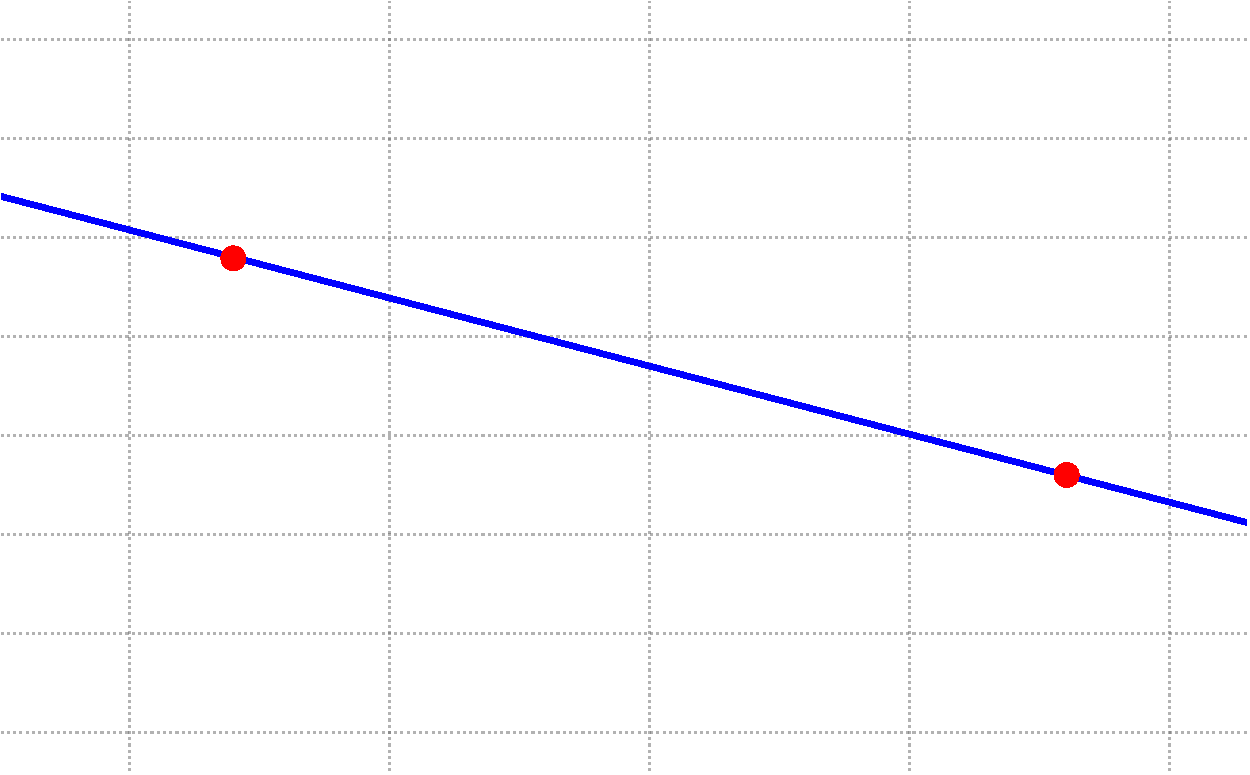
\includegraphics[width=0.8\textwidth]{images/lecture_1/simple_interpolation.pdf}
        \caption{$2$ points on the plane uniquely define the polynomial of degree $1$ (linear function).}
        \label{fig:simple_interpolation}
      \end{figure}
    \end{frame}

    \begin{frame}{Illustration with five points}
      \begin{figure}
        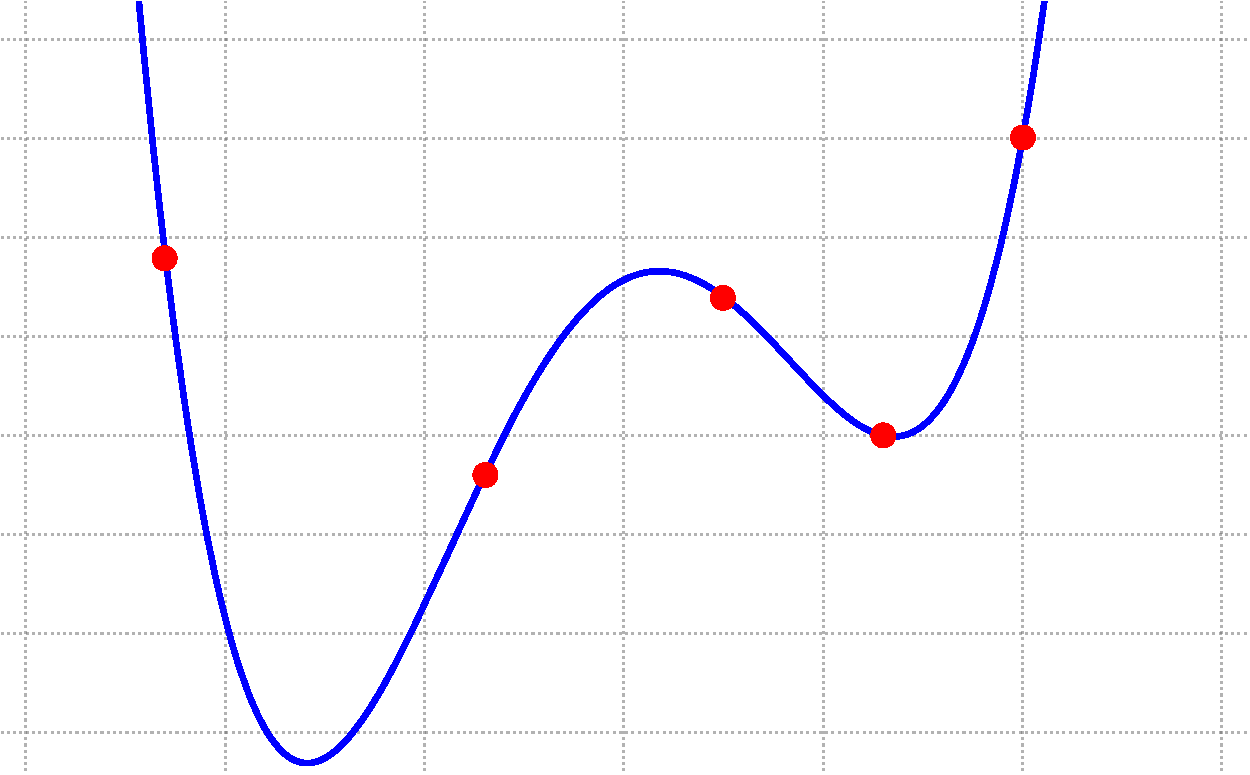
\includegraphics[width=0.8\textwidth]{images/lecture_1/interpolation.pdf}
        \caption{$5$ points on the plane uniquely define the polynomial of degree $4$.}
        \label{fig:interpolation}
      \end{figure}
    \end{frame}

    \begin{frame}{Illustration with three points}
      \begin{figure}
        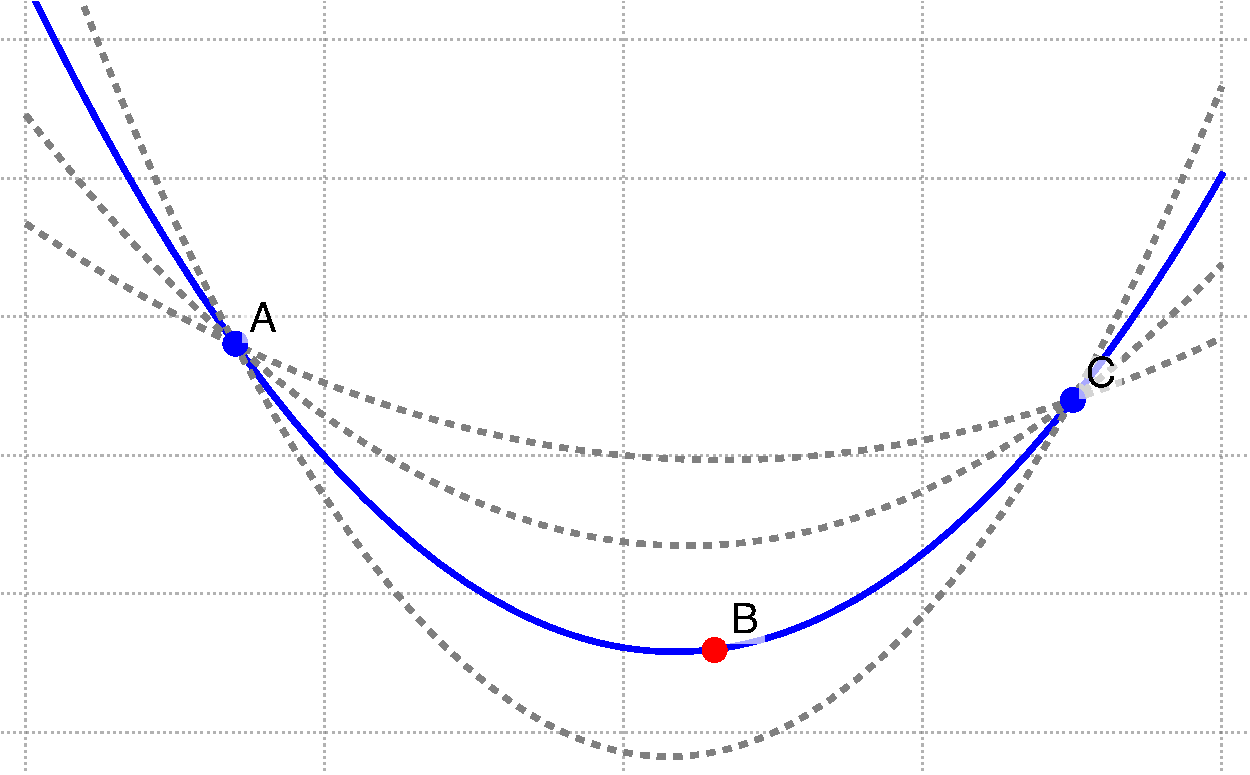
\includegraphics[width=0.8\textwidth]{images/lecture_1/shamir_demo.pdf}
        \caption{$2$ points are not enough to define the quadratic polynomial ($c_2x^2+c_1x+c_0$).}
        \label{fig:interpolation}
      \end{figure}
    \end{frame}

    \begin{frame}{Lagrange Interpolation}
      One of the ways to interpolate the polynomial is to use the Lagrange interpolation.

      \begin{theorem}
        Given $n+1$ distinct points $(x_0,y_0),\dots,(x_n,y_n)$, the polynomial $p(x)$ that passes through these points is given by
        \begin{equation*}
            p(x) = \sum_{i=0}^{n} y_i \ell_i(x), \quad \ell_i(x) = \prod_{i=0, j \neq i}^n \frac{x-x_j}{x_i-x_j}.
        \end{equation*}
    \end{theorem}
    \end{frame}

    \subsection{Interpolation Applications: Shamir Secret Sharing}
    \begin{frame}{Application: Shamir Secret Sharing}
      \begin{alertblock}{Motivation}    
        How to share a secret $\alpha$ among $n$ people in such a way that any $t$ of them can reconstruct the secret, but any $t-1$ cannot?
      \end{alertblock}  

      \begin{definition}
        \textbf{Secret Sharing} scheme is a pair of efficient algorithms $(\mathsf{Gen}, \mathsf{Comb})$ which work as follows:
        \begin{itemize}
            \item $\mathsf{Gen}(\alpha, t, n)$: probabilistic sharing algorithm that yields $n$ shards $(\alpha_1,\dots,\alpha_t)$ for which $t$ shards are needed to reconstruct the secret $\alpha$.
            \item $\mathsf{Comb}(\mathcal{I}, \{\alpha_i\}_{i \in \mathcal{I}})$: deterministic reconstruction algorithm that reconstructs the secret $\alpha$ from the shards $\mathcal{I} \subset \{1,\dots,n\}$ of size $t$.
        \end{itemize}
    \end{definition}
    \end{frame}

    \begin{frame}{Shamir's Protocol}
      \begin{block}{Note}
        Here, we require the \textbf{correctness}: for every $\alpha \in F$, for every possible output $(\alpha_1,\dots,\alpha_n) \gets \mathsf{Gen}(\alpha, t, n)$, and any $t$-size subset $\mathcal{I}$ of $\{1,\dots,n\}$ we have
        \begin{equation}
            \mathsf{Comb}(\mathcal{I}, \{\alpha_i\}_{i \in \mathcal{I}}) = \alpha.
        \end{equation}
      \end{block}

      \begin{definition}
        Now, \textbf{Shamir's protocol} works as follows: $F=\mathbb{F}_q$ and
        \begin{itemize}
            \item $\mathsf{Gen}(\alpha, k, n)$: choose random $k_1,\dots,k_{t-1} \xleftarrow[]{R} \mathbb{F}_q$ and define the polynomial
            \begin{equation}
                \omega(x) := \alpha + k_1x + k_2x^2 + \cdots + k_{t-1}x^{t-1} \in \mathbb{F}_q^{\leq (t-1)}[x],     
            \end{equation}
            and then compute $\alpha_i \gets \omega(i) \in \mathbb{F}_q, \; i = 1,\dots,n$. 
        \end{itemize}
      \end{definition}
    \end{frame}
  
    \begin{frame}{Shamir's Protocol}
      \begin{definition}
        \begin{itemize}
            \item $\mathsf{Comb}(\mathcal{I}, \{\alpha_i\}_{i \in \mathcal{I}})$: interpolate the polynomial $\omega(x)$ using the Lagrange interpolation and output $\omega(0) = \alpha$.
        \end{itemize}
      \end{definition}

      \begin{figure}
        \centering
        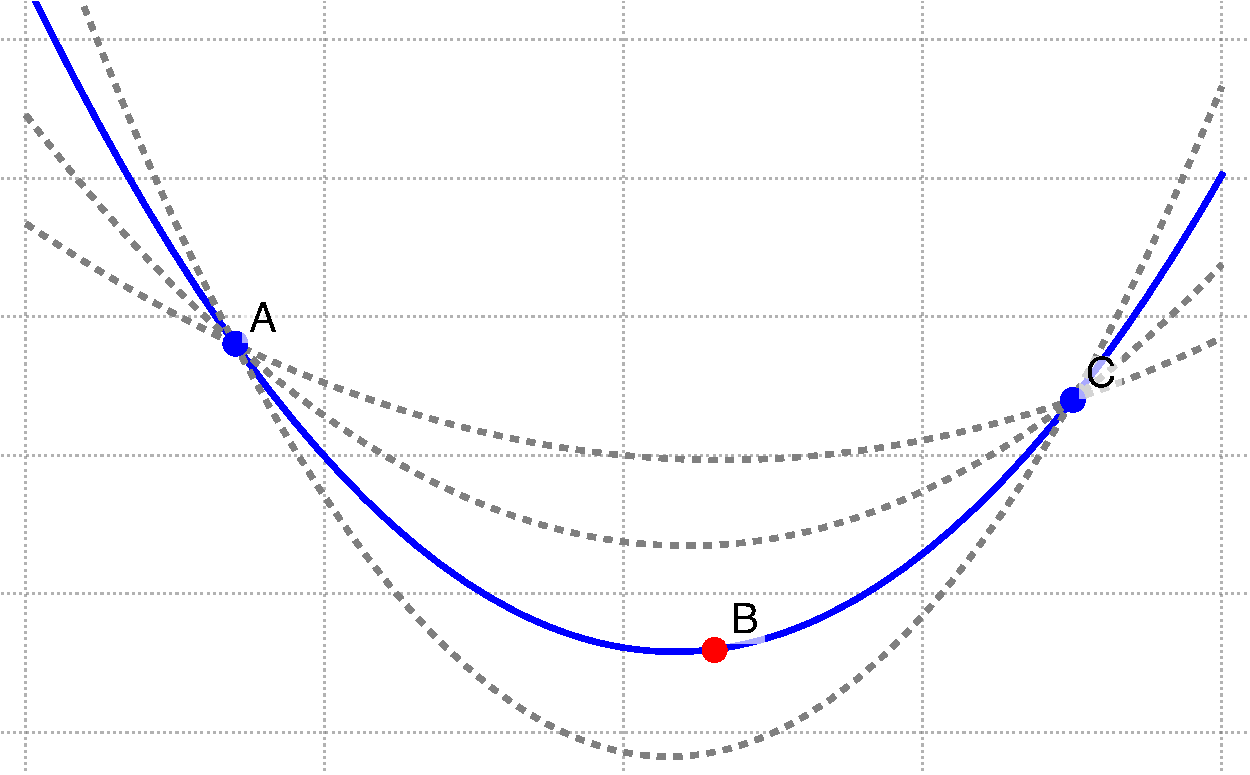
\includegraphics[width=0.5\textwidth]{images/lecture_1/shamir_demo.pdf}
        \caption{There are infinitely many quadratic polynomials passing through two \textcolor{blue}{blue} points (\textcolor{gray}{gray dashed} lines). However, knowing the \textcolor{red}{red} point allows us to uniquely determine the polynomial and thus get its value at $0$.}
        \label{fig:shamir}
      \end{figure}
    \end{frame}
  
    \begin{frame}{}
        \centering \Large
        \emph{Thanks for your attention!}
      \end{frame}
\end{document}